\section*{Circuito}

\begin{SCfigure}[1.5][h]
    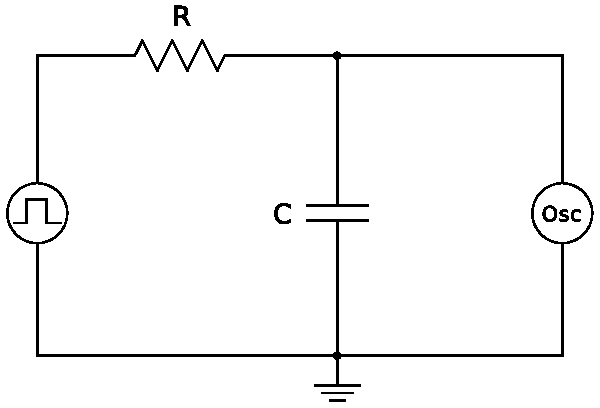
\includegraphics[width=60mm]{schema.pdf}
    \caption{Questo schema rappresenta il circuito utilizzato per questa sessione di laboratorio. Notiamo che la resistenza è in serie al parallelo tra il condensatore e l'osciloscopio. La diffrenza di potenziale fornita dal generatore d'onde è di $V\ped{0} \,=\, 1\,\si{\volt}$ e la frequenza che abbiamo deciso di utilizzare è di $20\,\si{\hertz}$. La funzione d'onda utilizzata è quella di un onda quadra in modo da approssimare il più possibile il generatore ad un interruttore.}
\end{SCfigure}

Facciamo notare che il circuito da noi utilizzato è alimentato da un'onda quadra che ci viene fornita dal generatore di forme d'onda. Questa configurazione è stata scelta al fine di sostituire un normale interruttore con il generatore di forme d'onda. Questo è stato fatto per poter ripetere ciclicamente il processo di carico e scarico del nostro condensatre.
La differenza di potenziale utilizzata è di $V\ped{0} \,=\, 1\,\si{\volt}$. Questa scelta è stata dettata dalla necessita di effettuare una rapida lettura del tempo caratteristico dall'oscilloscopio. Infine facciamo notare che abbiamo deciso di utilizzare una frequenza di $20\,\si{\hertz}$ per il generatore di funzioni d'onda al fine di ottenere un'immagine chiara e distinta dell'andamento della tensione in funzione del tempo sull'oscilloscopio.